\documentclass[a4paper, 12pt, compsoc]{IEEEtran}

\usepackage{amsmath}
\usepackage{physics}
\usepackage{hyperref}
\usepackage{cleveref}
\hypersetup{
	colorlinks = true,
	linkcolor = blue,
	filecolor = blue,
	citecolor = black,
	urlcolor = cyan,
}
\crefname{appsec}{Appendix}{Appendices}

\usepackage{graphicx}
\usepackage[section]{placeins}
\usepackage{bookmark}


%for code(MATLAB in particular)
\usepackage{listings}
\usepackage{color} %red, green, blue, yellow, cyan, magenta, black, white
\definecolor{mygreen}{RGB}{28,172,0} % color values Red, Green, Blue
\definecolor{mylilas}{RGB}{170,55,241}

\lstset{
    language=Matlab,%
    %basicstyle=\color{red},
    breaklines=true,%
    morekeywords={matlab2tikz},
    keywordstyle=\color{blue},%
    morekeywords=[2]{1}, 
    keywordstyle=[2]{\color{black}},
    identifierstyle=\color{black},%
    stringstyle=\color{mylilas},
    commentstyle=\color{mygreen},%
    showstringspaces=false,%without this there will be a symbol in the places where there is a space
    numbers=left,%
    numberstyle={\tiny \color{black}},% size of the numbers
    numbersep=7pt, % this defines how far the numbers are from the text
    emph=[1]{for,end,break},
    emphstyle=[1]\color{red}, %some words to emphasise
    %emph=[2]{word1,word2}, emphstyle=[2]{style},
}


\graphicspath{{./pictures/}}

\title{ECEN315 - Open Loop Response of a Motorised, Propellor Driven Pendulum}
\author{Joshua Benfell - 300433229}

% \IEEEtitleabstractindextext{
%     \begin{abstract}
        
%     \end{abstract}
% }


\begin{document}
    \maketitle
    \IEEEdisplaynontitleabstractindextext

    \section{Introduction}\label{sec:intro}
        This report covers the derivation of the theoretical open loop response for a motorised, propellor driven pendulum arm, for the purpose of later designing controllers. To do this the resultant angular displacement from an applied voltage needs to be quantifiable.

    \section{Background}\label{sec:bg}
        \begin{figure}[!h]
            \centering
            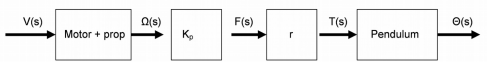
\includegraphics[width=\columnwidth]{overallBlockDiagram.png}
            \caption{Block diagram for full system}
            \label{fig:fullBlockDiagram}
        \end{figure}
        An open loop system is a system where the output is not fed back into the system. The alternative is a closed loop system where the input is fed back into the system, typically subtracted from the input to get the error. The full system (\cref{fig:fullBlockDiagram}) that this paper will be modelling can be done so as an open loop system. While the overarching system is an open loop system, some of the systems that make up the blocks are themselves, closed loop systems, while others are open loop systems.
        \par
        One of the evaluated characteristics of this system is it's stability. Stability of a system is defined as whether or not the output grows without bounds, if it does then the system is unstable, whereas it is stable if it settles on a value. This is regardless of any oscillation that would occur in the system. Stability can also be pre-determined by looking at the poles of the system, i.e. the values of $s$ that make the denominator of the transfer function $0$. If the real component of the poles is negative then the system is stable and vise versa if it is positive.
        \par
        The response of the system will be classified against a step input. This input is a suitable approximation for flicking a switch in a practical system.
        % \par
        % Design, solving, and evaluation of systems is typically done in the frequency domain.  


    \section{Method}\label{sec:methods}
        \begin{figure}[!h]
            \centering
            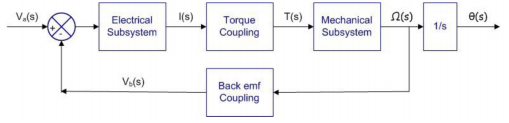
\includegraphics[width=\columnwidth]{motorTF.png}
            \caption{Block diagram that describes the motor response to an applied voltage. \cite{gouws_2008}}
            \label{fig:motorBlockDiagram}
        \end{figure}
        
        The block diagram in \cref{fig:fullBlockDiagram} illustrates an approximation of the full powered pendulum system. This system takes an input voltage into the motor causing the shaft to spin with angular velocity $\omega(t)$. Due to the propellor on the motor, this speed at which the shaft spins will generate a force which is represented by the constant $K_p$. The torque is then obtained by mutliplying by the distance from the pivot to the center of the motor. Finally this torque is applied to the pendulum arm, resulting in an angular displacement of the arm.
        \par

        \begin{figure}[]
            \centering
            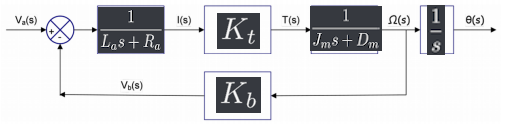
\includegraphics[width=\columnwidth]{full.png}
            \caption{Block diagram for motor and prop with equations in corresponding blocks \cite{gouws_2008}}
            \label{fig:motorBlockDiagramValues}
        \end{figure}
        The first block to look at is the one that describes how the motor responds to an applied voltage. This behaviour can be broken down into smaller sub-systems as shown in \cref{fig:motorBlockDiagram}.Each of those systems can be filled with the appropriate transfer function consisting of measurable properties of the motor with propellor as show in \cref{fig:motorBlockDiagramValues} where:
        \begin{itemize}
            \item $L_a$ is the inductance of the armature
            \item $R_a$ is the resistance of the armature
            \item $K_t$ is the torque constant that relates the current to the torque produced
            \item $J_m$ is the inertia of the load (propellor)
            \item $D_m$ is the damping coefficient of the load (propellor)
            \item $K_b$ is the back emf constant, relating the angular velocity to an induced voltage.
        \end{itemize}
        
        The block diagram can be simplified into a generic transfer function (\cref{eq:motorTF}) the represents the response of the motor to an applied voltage (See \cref{app:motorDerivation} for full derivation). This transfer function was then plugged into MATLAB and evaluated with step inputs of amplitude 2, 3, 4, 5 and 6V.
        \begin{equation} \label{eq:motorTF}
            \frac{\Omega(s)}{V(s)} = \frac{\frac{K_t}{J_mL_a}}{s^2  + \frac{J_mR_a + D_mL_a}{J_mL_a}s + \frac{R_aD_m+K_tK_b}{J_mL_a}}
        \end{equation}

        \begin{figure}[!h]
            \centering
            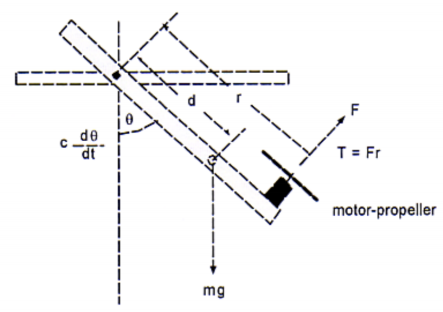
\includegraphics[width=\columnwidth]{pendulum.png}
            \caption{Diagram of the powered pendulum}
            \label{fig:pendulum}
        \end{figure}

        The next block to expand upon is the one that represents the pendulums response, as the two in the middle are just constants. For this block, a force is being applied (from the motor) which results in the angular displacement of the pendulum arm. An expression for net torque ($\tau_{net} = \alpha J_p$) must then be derived. Using the diagram in \cref{fig:pendulum}, it can be seen that there are three main torques acting on the arm; The torque from the propellored motor ($\tau_m = Fr$), the torque induced by friction around the pivot when the arm is moving ($\tau_f = c\dv{\theta}{t}$) and the component of the gravity vector that is perpendicular to the arm ($\tau_g = dmg\sin{\theta}$). 
        \par
        Combining the different torques of the system into one equation allows us to find an expression for the torque produced by the motor (\cref{eq:secondOrderDE}). After making the assumption that $\sin{\theta} = \theta$ and that $\alpha$ is the second derivative of angular displacement, \cref{eq:secondOrderDE} takes the form of a second order homogeneous ordinary differential equation. Applying the Laplace transform to this equation allows us to rearrange it so that it resembles a transfer function with angular displacement as the output to an applied torque (\cref{eq:pendulumTF}).

        \begin{equation}\label{eq:secondOrderDE}
            \begin{split}    
                \tau_{net} = & \tau_m - \tau_f - \tau_g \\
                \tau_m = & \tau_{net} + \tau_f + \tau_g \\ 
                \tau_m = & \alpha J_p + c\dv{\theta}{t} + dmg\sin{\theta} \\ 
                \tau_m =  & J_p \dv[2]{\theta}{t} + c\dv{\theta}{t} + dmg\sin{\theta} \\
                \tau_m =  & J_p \dv[2]{\theta}{t} + c\dv{\theta}{t} + dmg\theta
            \end{split}
        \end{equation}

        \begin{equation}\label{eq:pendulumTF}
            \frac{\Theta(s)}{\rm T(s)} = \frac{\frac{1}{J_p}}{s^2 + \frac{c}{J_p}s + \frac{dmg}{J_p}}
        \end{equation}

        Before plotting this in MATLAB for evaluation, the value for each variable need to be found. For $d$, $m$ and $g$ this is relatively easy as it is just measuring the distance to the center of mass, weighing it and using the constant value for gravity on earth of $9.81 \frac{m}{s^2}$. To find $J_p$ and $c$ the pendulum was let to fall and the oscillation recorded. An exponential was then fit through the peaks of the plot to find the values of $A$ and $B$ in \cref{eq:dampedPendulumEq} using the non-linear model (nlm) function in MATLAB (Can also see \cref{app:AB} for a manual method). \cref{eq:dampedPendulumEq} is the equation that models the motion of the pendulum where $\omega$ is given by \cref{eq:omega}. When finding $A$ and $B$, only the non-oscillitary component of \cref{eq:dampedPendulumEq} is important and used. Once found, \cref{eq:omega} can be rearranged for $J_P$ and then $c = 2BJ_p$.
        
        \begin{equation}\label{eq:dampedPendulumEq}
            \begin{split}
                y & = A e^{-\frac{c}{2J_p}t} \cos(\omega t + \phi) \\
                  & = A e^{-Bt}\cos(\omega t + \phi) 
            \end{split}
        \end{equation}

        \begin{equation}\label{eq:omega}
            \begin{split}
                \omega & = \sqrt{\frac{mgd}{J_p} - \left(\frac{c}{2J_p}\right)^2} \\ 
                  & = \sqrt{\frac{mgd}{J_p} - B^2}
            \end{split}
        \end{equation}

    \section{Results}\label{sec:results}
        \begin{table}
            \centering
            \caption{Table of Motor Parameters}
            \label{tab:motorValues}
            \begin{tabular}{l|r}
                Motor Parameters  & Value\\
                \hline
                $R_a (\Omega)$ & $6.3$\\
                $La (H)$ & $0.797$ \\
                $Kb (V.s/rad) = Kt (N.m/A)$ & $0.0043$ \\
                $Dm (N.m.s/rad)$ & $0.00000553$ \\
                $Jm (kgm2)$ & $0.00000241$
            \end{tabular}
        \end{table}
    \section{Discussion}\label{sec:discussion}
    \section{Conclusion}\label{sec:conclusion}


    \Urlmuskip=0mu plus 1mu\relax
    \bibliography{bibliography}
    \bibliographystyle{IEEEtran}

    \onecolumn
    \appendices
        \crefalias{section}{appsec}
        \section{Matlab Code}
            \lstinputlisting{../lab2.m}
            \lstinputlisting{../lab3.m}
        \section{Risk Assessment}

        \section{Derivation of the Motor Transfer Function}\label{app:motorDerivation}
            \begin{figure}[!h]
                \centering
                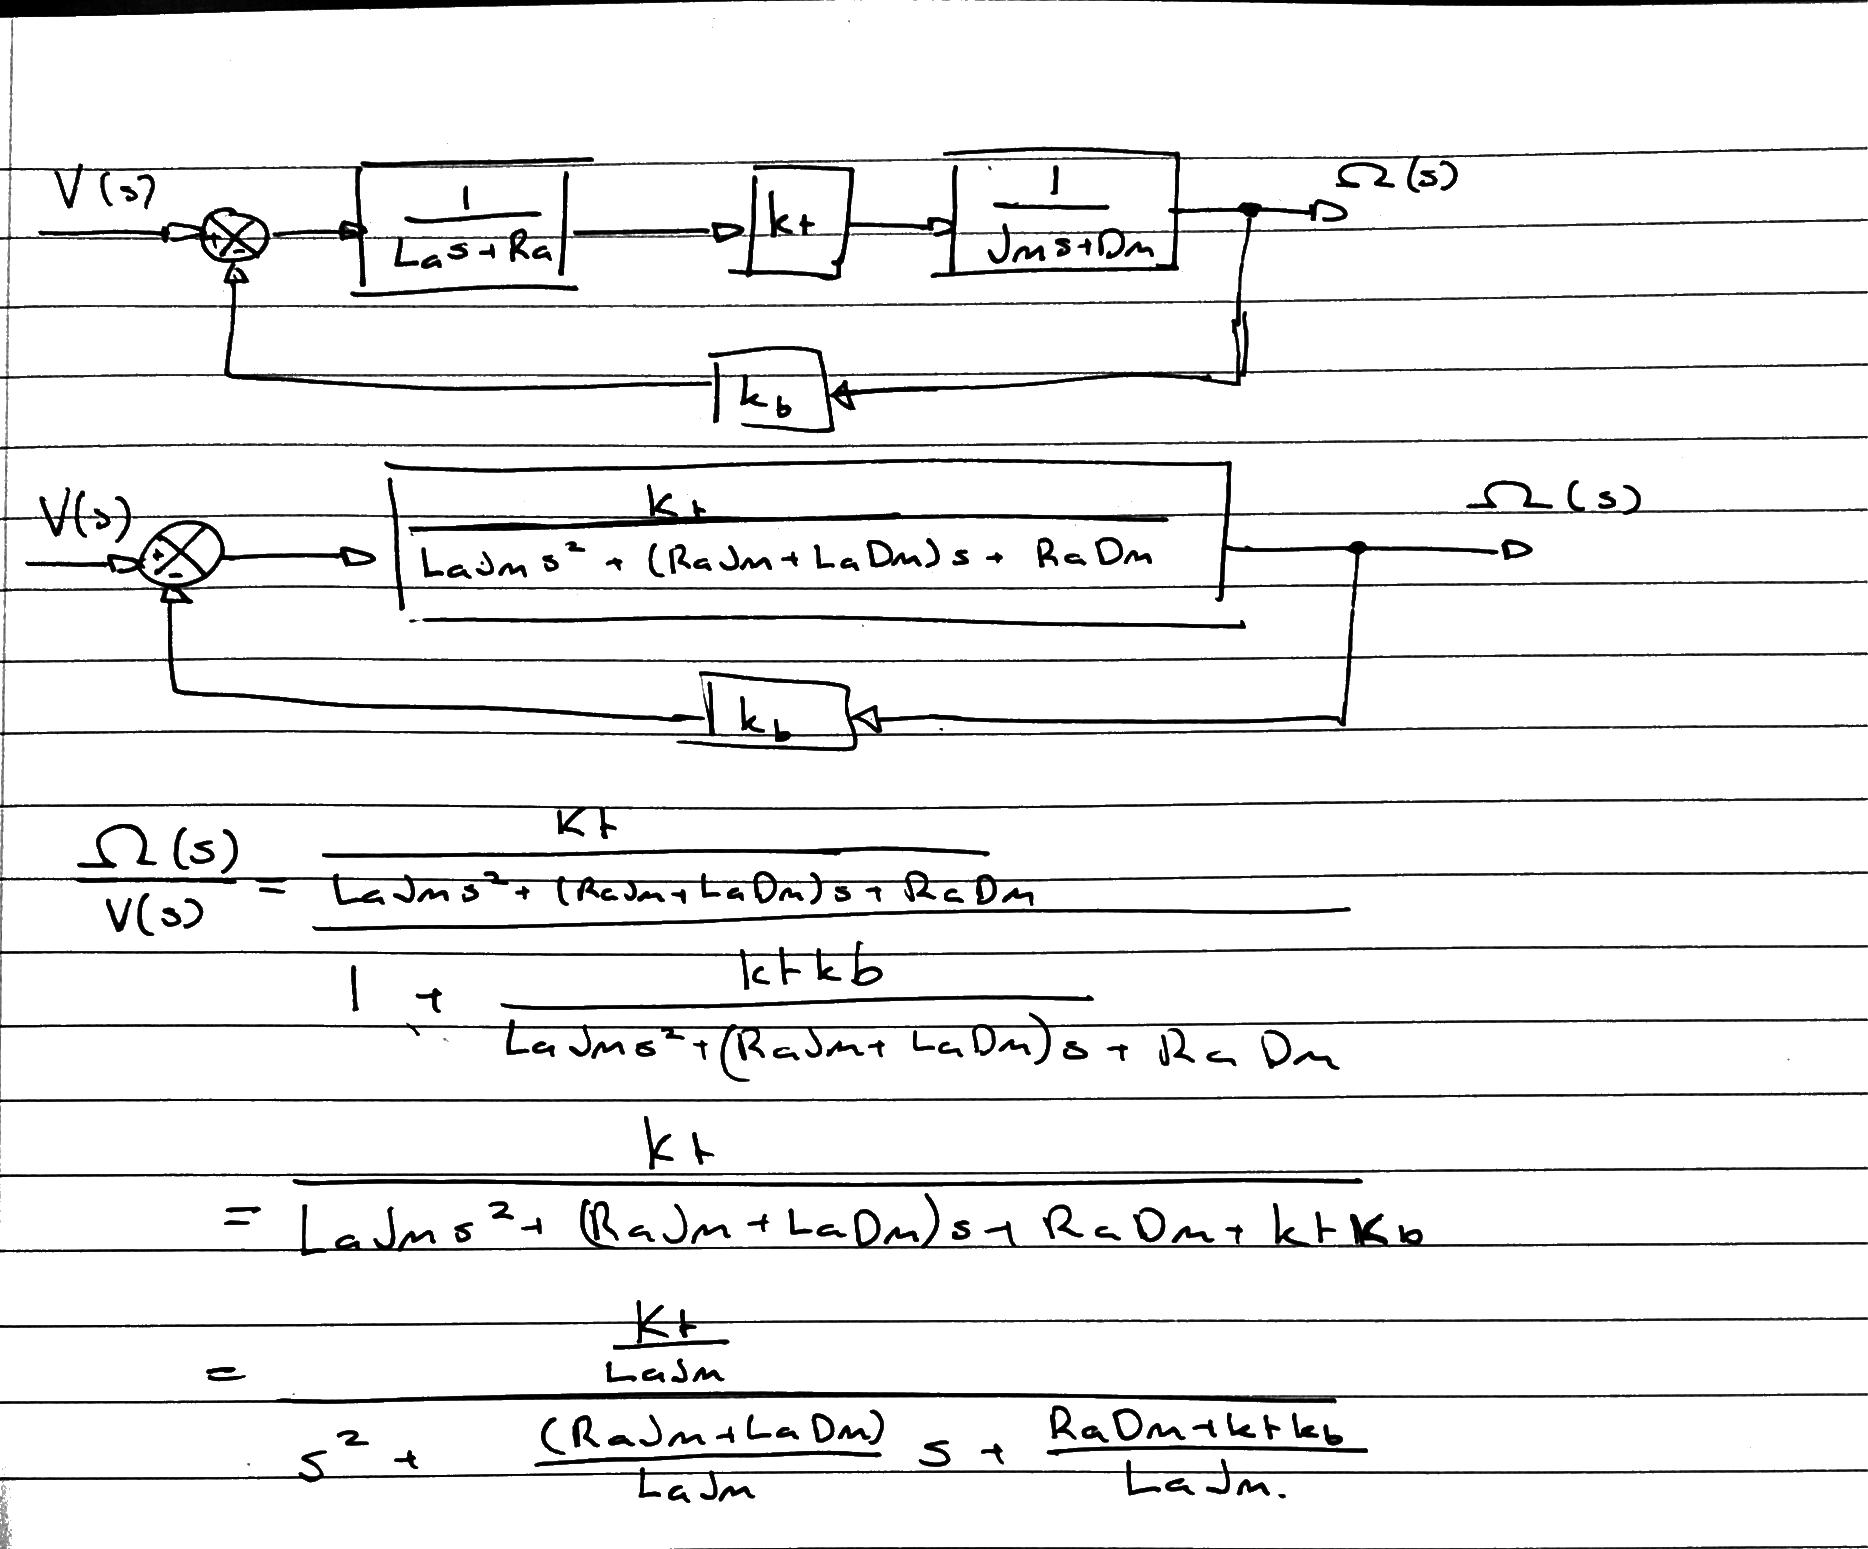
\includegraphics[width=\columnwidth]{lab2Derivation.jpg}
                \caption{Full derivation of \cref{fig:motorBlockDiagramValues} from block diagram to transfer function}
                \label{fig:motorDerivation}
            \end{figure}

        \section{Manaul Derivation of A and B for an Unpowered Damped Pendulum}\label{app:AB}
            \begin{figure}[!h]
                \centering
                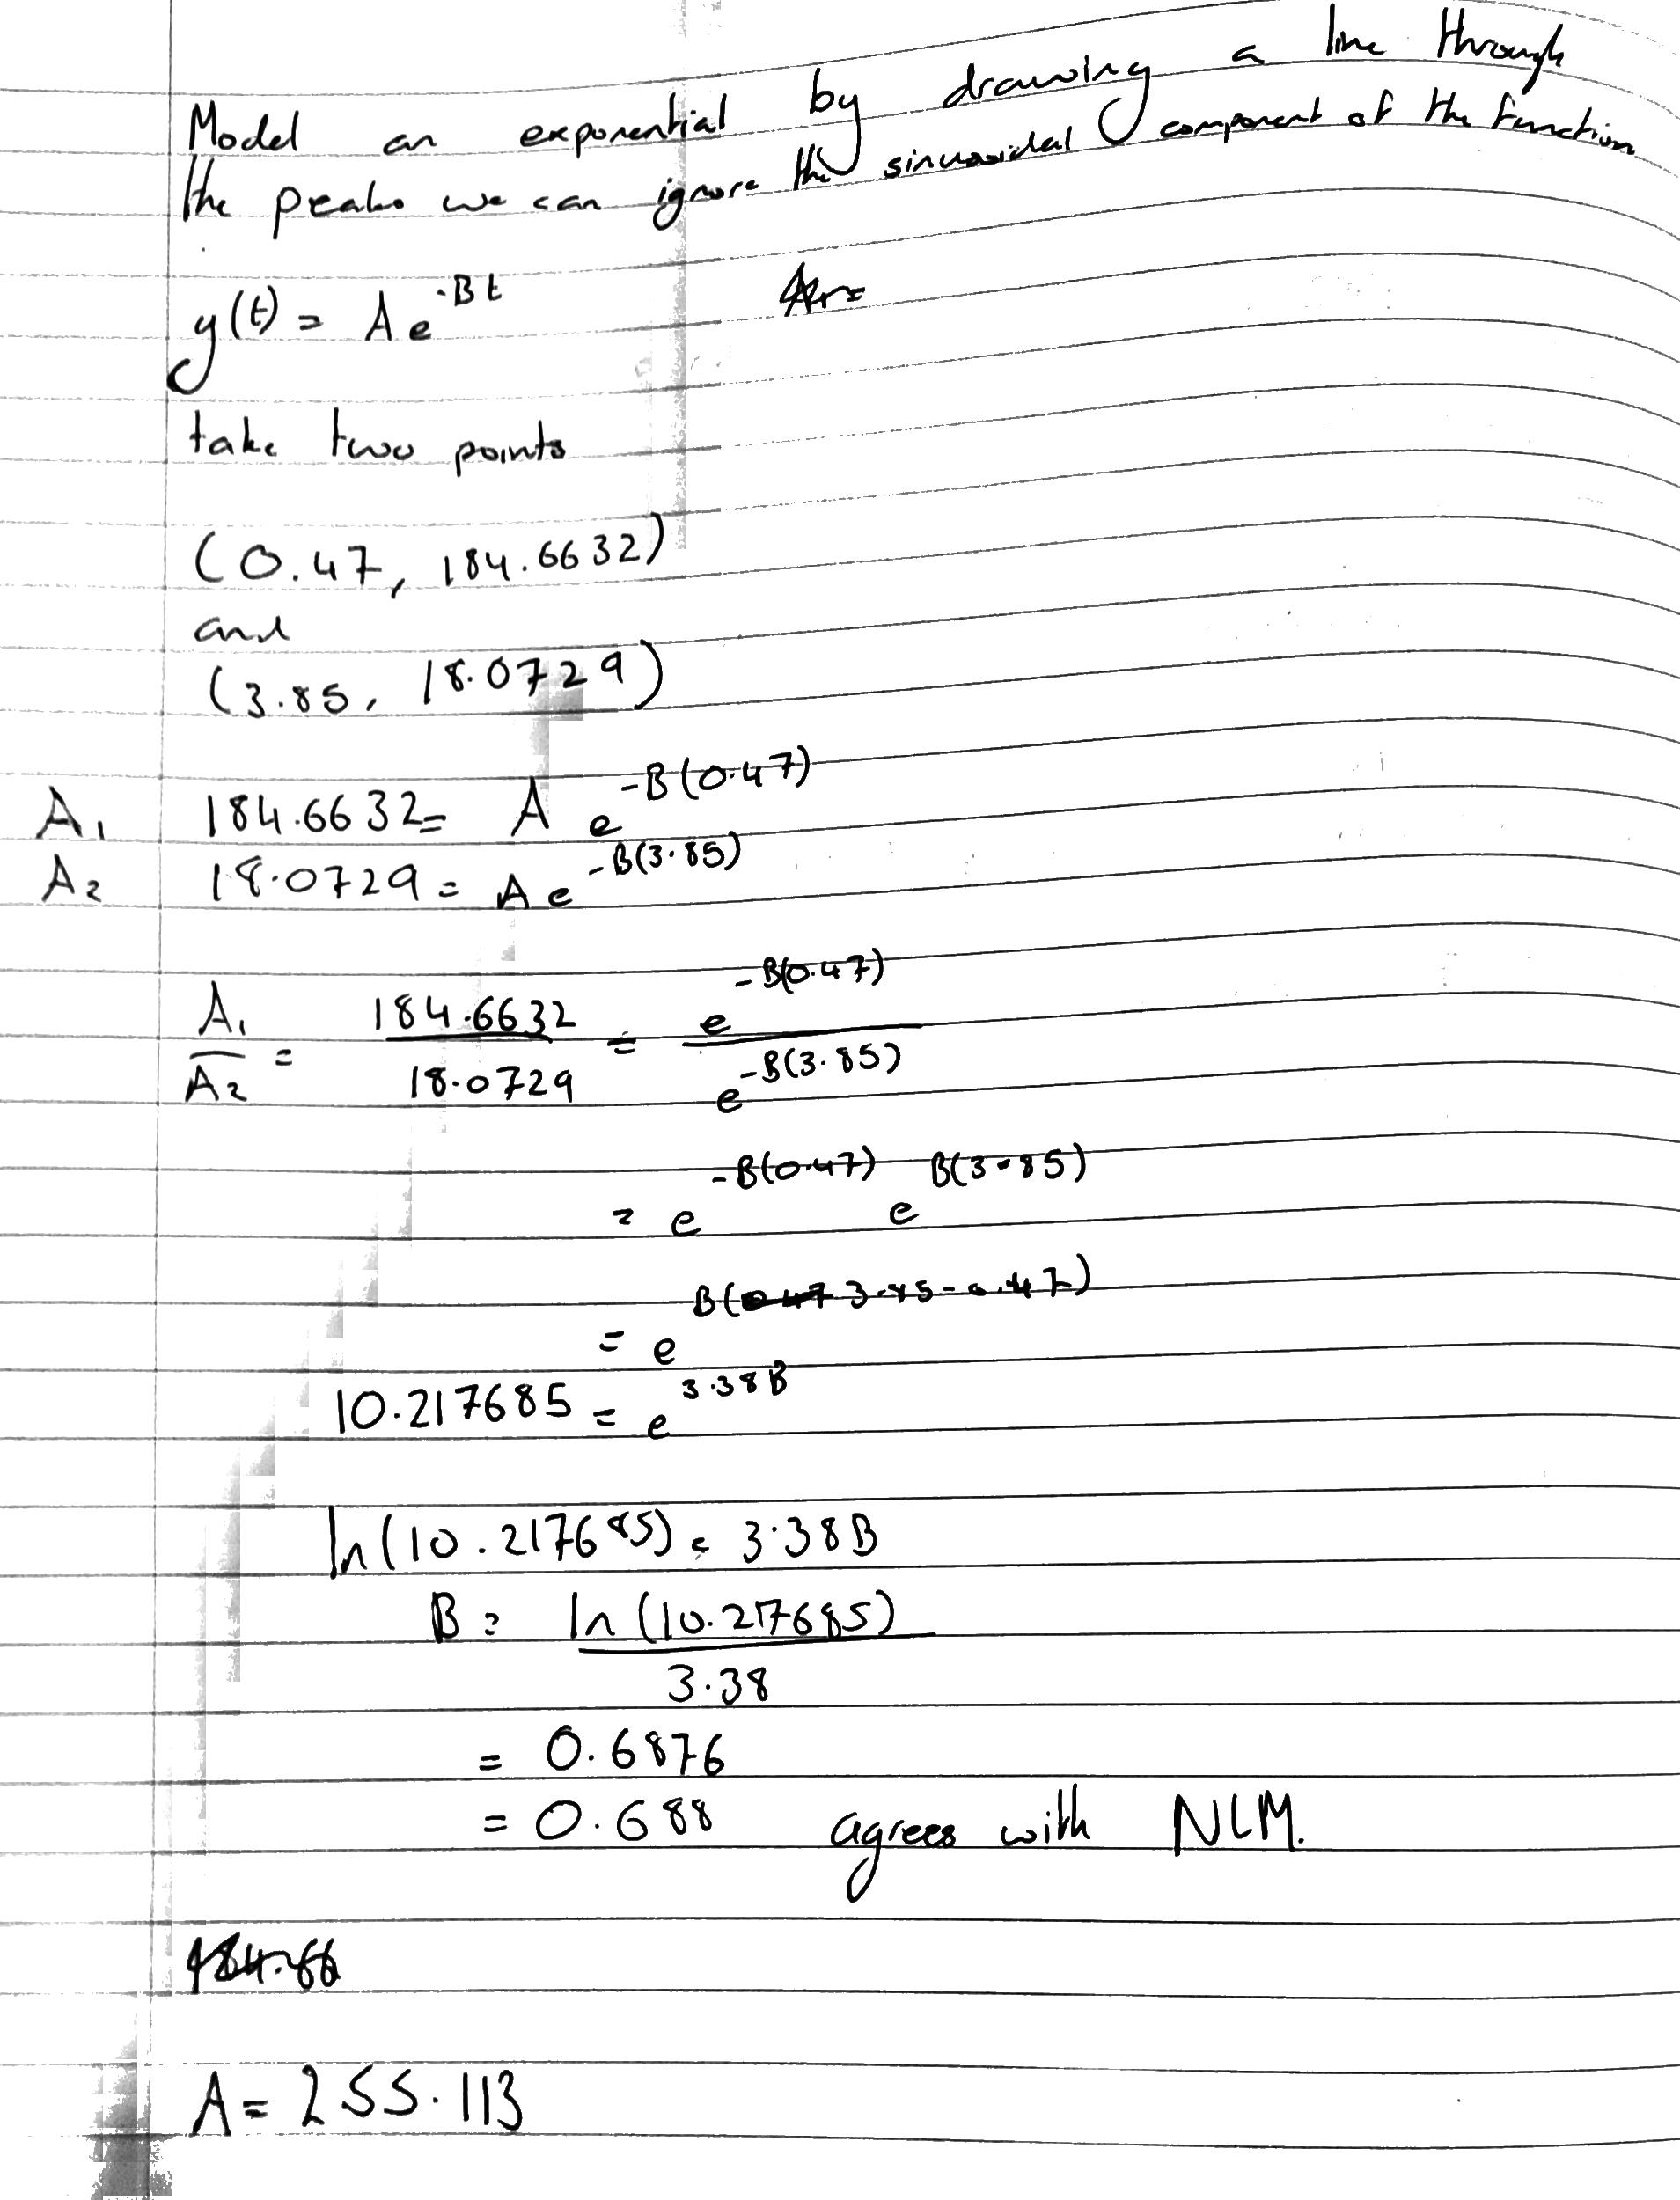
\includegraphics[width=0.9\columnwidth]{AB.jpg}
                \caption{Working for finding A and B using two peaks of a damped sinusoid}
                \label{fig:workingAB}
            \end{figure}

\end{document}